%-------------------------------
%	DOCUMENT SETTINGS
%-------------------------------
\documentclass[a4paper]{article}

\setlength{\hoffset}{-3.2cm}
\setlength{\voffset}{-3cm}
\setlength{\textwidth}{18.7cm}
\setlength{\textheight}{25.5cm}
\setlength{\parskip}{0pt}
\setlength{\parindent}{0in}

%----------------------------------------------------------------------------------------
%	PACKAGES AND OTHER DOCUMENT CONFIGURATIONS
%----------------------------------------------------------------------------------------

\usepackage{mathtools}
\usepackage{minted}
\usepackage[utf8]{inputenc} % Use UTF-8 encoding
\usepackage{microtype} % Slightly tweak font spacing for aesthetics
\usepackage[english]{babel} % Language hyphenation and typographical rules
\usepackage{amsthm, amsmath, amssymb} % Mathematical typesetting
\usepackage{float} % Improved interface for floating objects
\usepackage[final, colorlinks = true, 
linkcolor = black, 
\usepackage{dsfont}
%\DeclarePairedDelimiter\abs{\lvert}{\rvert}%
\usepackage{cancel}
\usepackage{blindtext} % Package to generate dummy text
\usepackage{charter} % Use the Charter font
\usepackage{graphicx, multicol} % Enhanced support for graphics
\usepackage{xcolor} % Driver-independent color extensions
\usepackage{marvosym, wasysym} % More symbols
\usepackage{rotating} % Rotation tools
\usepackage{censor} % Facilities for controlling restricted text
\usepackage{listings} % Environment for non-formatted code, !uses style file!
\usepackage{pseudocode} % Environment for specifying algorithms in a natural way
% Environment for f-structures, !uses style file!
\usepackage{booktabs} % Enhances quality of tables
\usepackage{tikz-qtree} % Easy tree drawing tool
% Configuration for b-trees and b+-trees, !uses style file!
%\usepackage[backend=biber,style=numeric,
%            sorting=nyt]{biblatex} % Complete reimplementation of bibliographic facilities
%\addbibresource{ecl.bib}
\usepackage{csquotes} % Context sensitive quotation facilities
%\usepackage[yyyymmdd]{datetime} % Uses YEAR-MONTH-DAY format for dates
\renewcommand{\dateseparator}{-} % Sets dateseparator to '-'
\usepackage{fancyhdr} % Headers and footers
citecolor = black]{hyperref} % For hyperlinks in the PDF
\pagestyle{fancy} % All pages have headers and footers
\fancyhead{}\renewcommand{\headrulewidth}{0pt} % Blank out the default header
\fancyfoot[L]{} % Custom footer text
\fancyfoot[C]{} % Custom footer text
\fancyfoot[R]{\thepage} % Custom footer text
\newcommand{\note}[1]{\marginpar{\scriptsize \textcolor{red}{#1}}} % Enables comments in red on margin

%----------------------------------------------------------------------------------------
%	CUSTOM COMMANDS
%----------------------------------------------------------------------------------------

\newcommand{\R}{\mathbb{R}}
\newcommand{\E}{\mathbb{E}}
\newcommand{\I}{\mathbb{I}}
\newcommand{\Var}{\text{Var}}
% Para poner sonrisa sobre puntos suspensivos. Uso: \overplace{n}{\dotsc}
\newcommand{\overplace}[2]{%
	\overset{\substack{#1\\\smile}}{#2}%
}

\begin{document}
	
%-------------------------------
%	TITLE SECTION
%-------------------------------

\fancyhead[C]{}
\hrule \medskip % Upper rule
\begin{minipage}{0.295\textwidth} 
	\raggedright
	\footnotesize
	José Antonio Álvarez Ocete \hfill\\   
	77553417Q \hfill\\
	joseantonio.alvarezo@estudiante.uam.es
\end{minipage}
\begin{minipage}{0.4\textwidth} 
	\centering 
	\large 
	Entrega final\\ 
	\normalsize 
	Procesos estocásticos discretos\\ 
\end{minipage}
\begin{minipage}{0.295\textwidth} 
	\raggedleft
	\today\hfill\\
\end{minipage}
\medskip\hrule 
\bigskip

%-------------------------------
%	CONTENTS
%-------------------------------

\section*{Ejercicio I.}

\textbf{Enunciado.} En los apuntes hay el ejemplo del *gambler's ruin* como cadena de Markov:

\begin{figure}[H]
	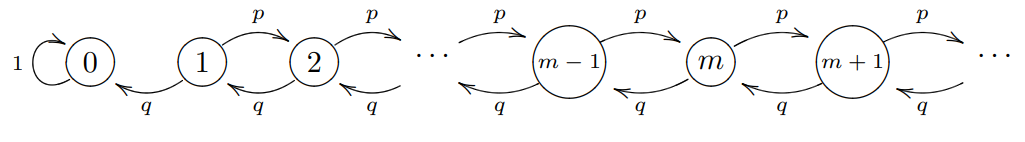
\includegraphics[scale=.14]{figures/gamblers_ruin}
	\centering
\end{figure}

Donde estar en el nodo $i$ implica tener $i$ Euros, y $p$ y $q=1-p$ son las probabilidades de ganar en cada repetición del juego.

\textbf{a)} Hacer un gráfico del número medio de jugadas que el jugador puede hacer antes de arruinarse en función del dinero inicial. En cada jugada se juega $1$ Euro, y el juego es ecuo (el jugador tiene una probabilidad $p=1/2$ de ganar).

Sabemos por el estudio teórico realizado para este problema que en el caso de $p=q=\frac{1}{2}$, el jugador convergerá a arruinarse tarde o temprano. Sin embargo, la simulación puede tomar un tiempo arbitrariamente alto de tiempo si el dinero inicial es alto. Es por ello que hemos de poner un límite al número de iteraciones máximo que ejecutaremos nuestra simulación. Consideramos que $10^5$ es una cantidad aceptable de iteraciones para los bajos valores de dinero inicial que utilizaremos. Si se alcanza ese número de iteraciones podemos considerar que el jugador "se arruina en tiempo $10^5$, que es básicamente infinito.

Implementamos la simulación de esta cadena de Markov y la ejecutamos $20$ veces, computando su media. Realizar esta simulación en múltiples ocasiones y utilizar la media es imprescindible para obtener resultados representativos en procesos de Monte Carlo como este.
	
\begin{minted}{python}
def simulate_gambler_step(p=1/2):
	""" 
		Simulates a single step of the gambler's ruin
		- p: the probability of winning
		- returns: 1 if won, -1 if lost
	"""
	r = random.uniform(0, 1)
	return 1 if r <= p else -1

def simulate_gamblers_ruin(initial_money, p=1/2, max_steps=10**6):
	"""
		Simulates a gambler's ruin markov chain.
		- initial_money: the starting node
		- p: the probability of winning at each step
		- max_steps: the max number of steps to be comptued
		- returns: time taken to ruin the gambler. If max_steps is reached
		without ruining the gambler, return max_steps instead.
	"""
	money = initial_money
	steps = 0
	while money > 0 and steps <= max_steps:
	steps += 1
	money += simulate_gambler_step(p)
	return steps

def plot_mean_ruin_time(max_initial_money=50, n=20, max_steps=10**5, p=1/2):
	"""
		Plots the mean time for a gambler's to ruin themself, against the initial money.
		- max_initial_money: max initial money to be plotted
		- n: the number of executions per initial money value
		- max_steps: the max number of steps to be comptued
		- p: the probability of winning at each step
	"""
	# Compute times
	initial_money_range = np.arange(1, max_initial_money)
	mean_times = [
		np.mean( [simulate_gamblers_ruin(initial_money, p=p, max_steps=max_steps)
				for _ in range(n)] )
		for initial_money in initial_money_range
	]

	# Plotting
	plt.figure(figsize=(12,6))
	plt.plot(initial_money_range, mean_times, '-o')
	plt.legend(['Mean time to ruin', 'Max iterations'])
	plt.xlabel('Initial money')
	plt.ylabel('Mean time to ruin in {} iterations'.format(n))
	plt.title('Gambler\' ruin simulation')
	plt.show()
	
random.seed(123)
plot_mean_ruin_time(max_steps=10**5)
\end{minted}
	
\begin{figure}[H]
	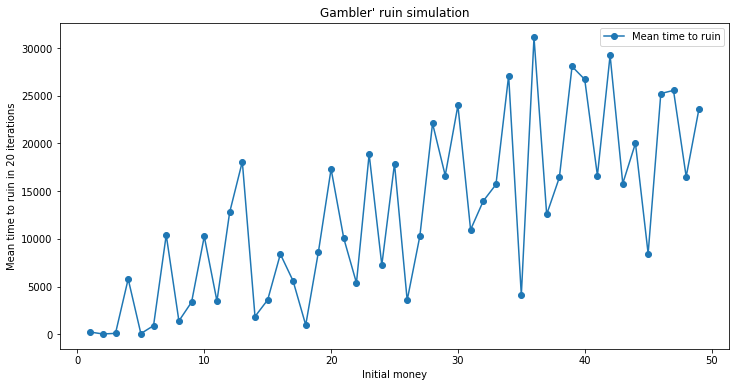
\includegraphics[scale=.14]{figures/gambler1}
	\centering
	\caption{Single simulation of Gambler's Ruin problem}
\end{figure}


\end{document}
